\section{Introduction}
    In this implementation, in order to demonstrate how the monitoring system works instead of using actual sensors, a data generator has been used and it simulates reading of sensors (such as humidity, temperature and electricity).

\section{Methodology}
A data generator should have a random yet realistic pattern for effective system testing, so just using a simple random number would be insufficient. Therefore, in this thesis a controlled version of choosing a random number was used to mimic some parts of real-world criteria and avoid sudden changes. The methodology for this process can be seen in the accompanying flowchart \ref{chart:data_gen}.

    \begin{figure}
        \centering
        \captionsetup{type=figure}
        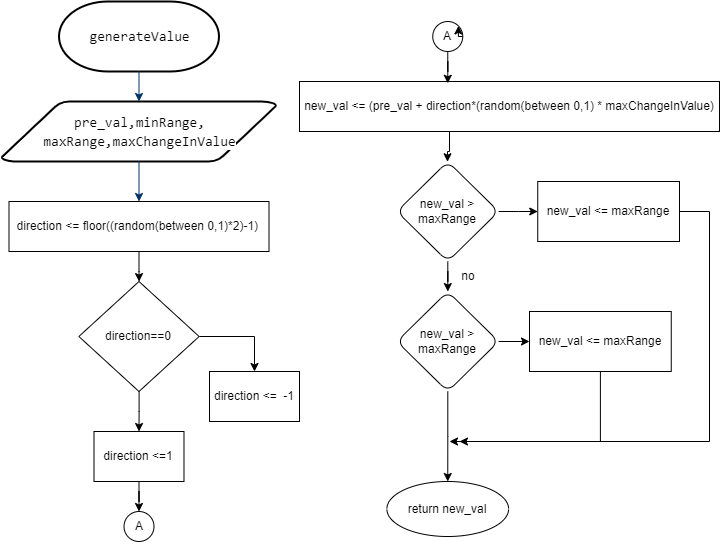
\includegraphics[width=1\textwidth]{flowchart_data_gen}
        \caption{Flowchart of data generator}
        \label{chart:data_gen}
    \end{figure}
\section{Results}
    As discussed in the methodology section, the program was implemented, and the generated values tested with different parameters was saved and reported as line charts in the subsequent sections.
    \subsection{Generated data for temperature sensor}
        \begin{itemize}
            \item Parameters
                \begin{description}
                    \item[Minimum Posible Temperature:] 18
                    \item[Maximum Posible Temperature:] 27
                    \item[Maximum Posible Change in an iteration:] 0.5
                \end{description}
            \item Results can be seen in line graph \ref{chart:gen_temperature}
                \begin{figure}
                    \centering
                    \captionsetup{type=figure}
                    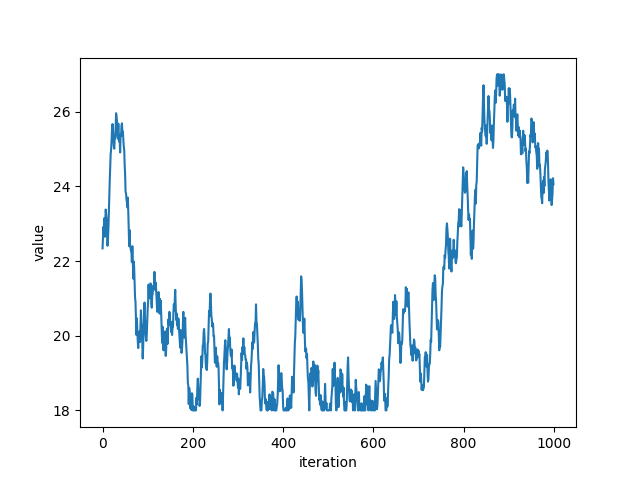
\includegraphics[width=1\textwidth]{linechart_data_gen_temperature}
                    \caption{Generated data for 1000 iterations}
                    \label{chart:gen_temperature}
                \end{figure}
        \end{itemize}
